\documentclass[a4paper, 12pt]{article}
\usepackage[utf8]{inputenc}  % Unicode
\usepackage[french]{babel}
\usepackage{geometry}
\usepackage{graphics}
\usepackage[pdftex]{graphicx, color}
\usepackage{pdfpages}
\DeclareGraphicsExtensions{.jpg,.png}
\pdfoutput=1
\usepackage[pdftex,
	bookmarks = true,           % Signets
	bookmarksnumbered = true,   % Signets numerotes
	pdfstartview = FitV,        % La page prend toute la hauteur
	colorlinks=true,
	citecolor=black,urlcolor=blue,linkcolor=black,
	pdfauthor={Auteur},
	pdftitle={Titre},
 	pdfsubject={Sujet},
%	pdfkeywords={},	% Besoin de keywords ?
	plainpages=false,
	pdfpagelabels,
	breaklinks=true,
   	hyperindex,
	linktocpage=true	% pour colorier seulement le numéros dans la TOC	
]{hyperref}
\usepackage{float}
\usepackage{listings}
\usepackage{alltt}
\usepackage{amsmath}
\renewcommand{\ttdefault}{txtt}

\lstset{basicstyle=\ttfamily,
escapeinside={||},
mathescape=true}
\setcounter{secnumdepth}{3}
\newcommand{\HRule}{\rule{\linewidth}{0.5mm}}

\newcommand*\styleC{\fontsize{9}{10pt}\selectfont }
\newcommand*\styleD{\fontsize{9}{10pt}\usefont{OT1}{pag}{m}{n}\selectfont }

\makeatletter
% on fixe le langage utilisé
\lstset{language=matlab}
\edef\Motscle{emph={\lst@keywords}}
\expandafter\lstset\expandafter{
}
\makeatother



\definecolor{Ggris}{rgb}{0.45,0.48,0.45}

\lstset{emphstyle=\ttfamily\color{blue}, % les mots réservés de matlab en bleu
basicstyle=\ttfamily\styleC, % 
keywordstyle=\ttfamily,
commentstyle=\color{Ggris}\styleD, % \styleD commentaire en gris
numberstyle=\tiny\color{black},
numbers=left,
numbersep=10pt,
lineskip=0.7pt,
showstringspaces=false}
%  % inclure le fichier source
\newcommand{\FSource}[1]{%
\lstinputlisting[texcl=true]{#1}
}

%%%%%%%%%
\textwidth=15cm
\textheight=21cm
%\hoffset=-2.5cm
\tolerance=9000
\hbadness=9000
\pretolerance=2500


\begin{document}
%\rmfamily

\begin{titlepage}
\begin{center}



\textsc{\Large Rapport de TP - SY26}\\[0.5cm]
\vspace{4cm}
% Title
\HRule \\[0.4cm]
{ \huge \bfseries TP02 - Codage de Huffman \\[0.4cm] }

\HRule \\[1.5cm]

% Author and supervisor
\begin{minipage}{0.4\textwidth}
\begin{flushleft} \large
R\'emi \textsc{Burtin}
\end{flushleft}
\end{minipage}
\begin{minipage}{0.4\textwidth}
\begin{flushright} \large
Cyril \textsc{Fougeray}
\end{flushright}
\end{minipage}

\vspace{4cm}

{\large \today}



\vfill
% Bottom

\includegraphics[width=0.25\textwidth]{logo.jpg}\\[0.5cm]

\textsc{\LARGE Universit\'{e} de Technologie de Compi\`{e}gne}\\[1.5cm]


\end{center}
\end{titlepage}


%\begin{abstract} 
%\end{abstract} 

%{\bf Keywords:} \newline


\clearpage

\section{Introduction}

Le but de ce TP est de mettre en œuvre la technique du \textit{block matching} utilisée dans certains algorithmes de compression vidéo (codage inter-image, \textit{P-Frame}).

Le principe est le suivant : l’image courante est divisée en blocs de taille MxM. On définit dans l’image de référence une zone de recherche de taille 2W+M placée autour de la position du centre du bloc de l’image courante. Chaque bloc dans la zone de recherche est ensuite comparé avec le bloc de l’image courante (on utilisera ici le critère \textit{Mean Squared Difference}).


\section{Mise en oeuvre du block matching}

\subsection{Padding de l'image}

La division de l'image en bloc implique que la largeur et la hauteur de l'image soient respectivement multiples de la largeur et de la hauteur des blocs. Si ce n'est pas le cas, nous complétons avec des zéros (pixels noirs) grâce à la fonction \textbf{padarray} et son paramètre DIRECTION que nous fixons à 'post' afin d'ajouter les pixels après. Pour calculer le nombre de pixels à rajouter en largeur on utilise la formule suivante : \\

\begin{center}
	$(M - (largeur(image) \mod M)) \mod M$ \\
\end{center}
avec M largeur d'un bloc = $2^N + 1$, N un entier.\\
Dans le cadre de cet exercice nous faisons varier N entre 1 et 3.\\

\textit{NB.} Afin de simplifier les calculs, nous convertissons les images en niveaux de gris afin de les manipuler plus aisément.

\begin{figure}[H]
	\centering
		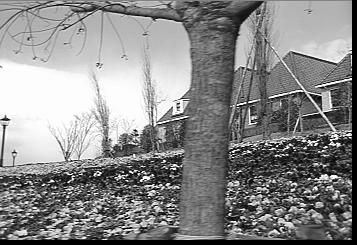
\includegraphics[height=6cm]{../Resultats/Garden/garden_padding.jpg}
	\caption{Image, issue de la video \textit{garden}, que l'on a voulu diviser en bloc de 7x7. L'image faisant 352x240, il a fallu rajouter 5 pixels noirs en largeur et 5 en hauteur.}
	\label{fig:padding}
\end{figure}

\subsection{Calcul de la fenêtre de recherche}

Pour chaque bloc de l'image, nous devons maintenant calculer une fenêtre de recherche centrée sur le bloc courant et d'une taille de $2W+M$ (W prendra les valeurs 5, 10 et 15 dans notre cas). Afin de calculer les coordonnées de cette fenêtre pour chacun des blocs, nous parcourons tout d'abord tous ces blocs grâce à l'imbrication de deux boucles, ce qui nous permet de calculer les coordonnées du premier pixel dans le coin supérieur gauche du bloc puis de calculer la fenêtre de recherche via la fonction \textit{search\_window} (\textit{cf.} \ref{search_window}) :
\begin{alltt} 
% Pour i allant de 1 à hauteur de l'image, par pas de M.
for i=1:M:size(img,1), 
	% Pour i allant de 1 à largeur de l'image, par pas de M.
	for j=1:M:size(img,2),
		% extraction bloc courant
		block = img(i:i+M-1,j:j+M-1);
		%calcul de la fenetre de recherche
		[window, orig_x, orig_y] = search_window(img_ref,W,M,i,j);
		[...]
	end;
end;
\end{alltt}

La fonction \textit{search\_window} renvoie trois paramètres : 
\begin{itemize}
  \item \textit{window} : matrice constituée des pixels de la fenêtre de recherche
  \item \textit{orig\_x} : coordonnée en x du bloc courant dans la fenêtre de recherche
  \item \textit{orig\_y} : coordonnée en y du bloc courant dans la fenêtre de recherche
\end{itemize}

Afin de calculer les coordonnées dans l'image de la fenêtre de recherche, nous ajoutons (resp. soustrayons) W aux coordonnées horizontales et verticales des bords droit et bas (resp. gauche et haut) du bloc courant, tout en faisant attention à les coordonnées calculées ne débordent pas de l'image.


\subsection{Recherche du meilleur bloc}

Pour la recherche du bloc le plus similaire compris dans la fenêtre de recherche, nous avons créé une fonction prenant en paramètre le bloc, la fenêtre ainsi que les coordonnées du bloc dans la fenêtre (\textit{cf.} § précédent).\\

Le but est de trouver le vecteur de mouvement telle que l'erreur moyenne, calculé via le critère MSD, soit minimale. Nous avons mis en place une méthode de recherche complète (dans toute la fenêtre) ce qui est une solution lente à exécuter mais simple à mettre en œuvre, comparé à la méthode de recherche logarithmique à deux dimensions ou à l'estimation de mouvement dite hiérarchique. Le but ici est donc de parcourir toute la fenêtre avec le bloc courant : nous implémentons cette étape grâce à deux boucles imbriquées afin de parcourir les lignes et les colonnes. Pour chaque position du bloc dans la fenêtre de recherche, nous calculons le MSD. Nous avons pour cela implémenté un fonction, \textit{compute\_msd} (\textit{cf.} \ref{msd_code}). Cette fonction implémente la formule suivante (C étant le bloc dans l'image courante, P dans l'image prédite) :
\[ MSD = \frac{1}{M^2}\sum_{i=0}^{M-1}\sum_{j=0}^{M-1}(C(i,j) - P(i,j))^2 \]

Nous sauvegardons le minimum de tous les MSD calculés ainsi que le vecteur de mouvement pour le bloc correspondant.

\subsection{Reconstruction image prédite}

Nous construisons l'image prédite à partir des blocs de l'image de référence. Le bloc $ij$ de l'image prédite correspondra au bloc de l'image de référence (que nous avons trouvé lors de l'étape précedente) qui correspond le mieux au bloc $ij$ de l'image courante. Pour récupérer ces bloc, nous utilisons les vecteurs de déplacement calculés précédemment : 

\begin{alltt} 
ref_block = img_ref(i+delta_y : i+M-1+delta_y ,j+delta_x : j+M-1+delta_x);
output_image(i : i+M-1 ,j : j+M-1) = ref_block;
\end{alltt}

\newpage
\section{Résultats}

Pour montrer nos résultats, nous allons utiliser deux images issue de la séquence garden (très utilisée dans le domaine du traitement vidéo, comme Lena pour le traitement des images). Voici les deux images que nous allons utiliser : 

\begin{figure}[H]
	\centering
	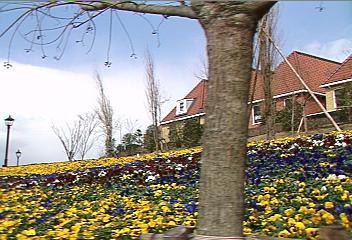
\includegraphics[height=5cm]{../garden1.jpg}
	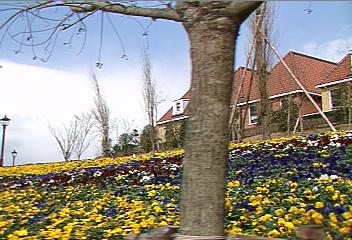
\includegraphics[height=5cm]{../garden2.jpg}
	\caption{Frames 2 et 5 de la séquence garden}
	\label{fig:garden}
\end{figure}

Le MSD entre ces deux images s'élève à 3465. Voici l'image résultante de la différence entre l'image courante (Frame 5) et l'image de référence (Frame 2) :

\begin{figure}[H]
	\centering
	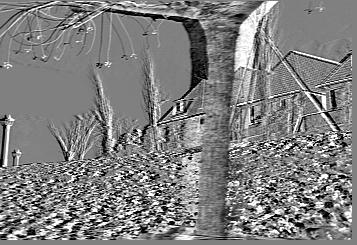
\includegraphics[height=7cm]{../Resultats/Garden/garden_error.jpg}
	\caption{Différence entre image courante et image de référence}
	\label{fig:garden_error}
\end{figure}

On commence par un effectuer un block matching avec des blocs d'une taille 7x7 et une fenêtre de recherche de 17x17 (ou moins selon la position du bloc courant dans l'image) :

\begin{figure}[H]
	\centering
	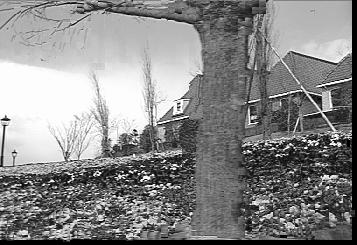
\includegraphics[height=5cm]{../Resultats/Garden/garden_pred_n_3_w_5.jpg}
	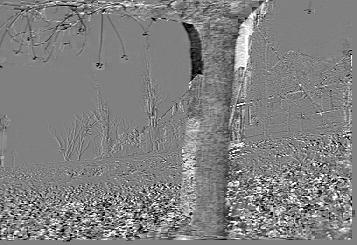
\includegraphics[height=5cm]{../Resultats/Garden/garden_error_n_3_w_5.jpg}
	\caption{Image courante prédite et erreur de prédiction pour $N=3$ et $W=5$. Le MSD est alors de 1128.}
	\label{fig:garden_3_5}
\end{figure}

On passe ensuite à des blocs 3x3 et une fenêtre de recherche 33x33. On devra donc analyser beaucoup plus de positions mais la prédiction sera beaucoup plus fine. En effet on voit que le MSD tombe à 188 :

\begin{figure}[H]
	\centering
	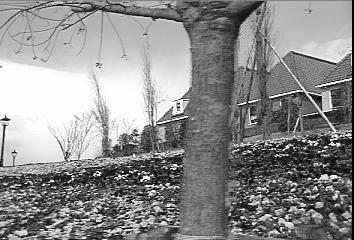
\includegraphics[height=5cm]{../Resultats/Garden/garden_pred_n_1_w_15.jpg}
	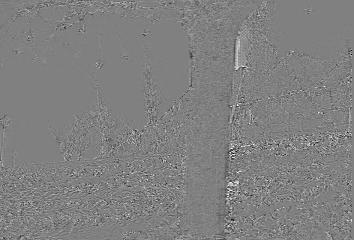
\includegraphics[height=5cm]{../Resultats/Garden/garden_error_n_1_w_15.jpg}
	\caption{Image courante prédite et erreur de prédiction pour $N=1$ et $W=15$. Le MSD tombe alors à 188.}
	\label{fig:garden_1_15}
\end{figure}

\begin{figure}[H]
	\centering
	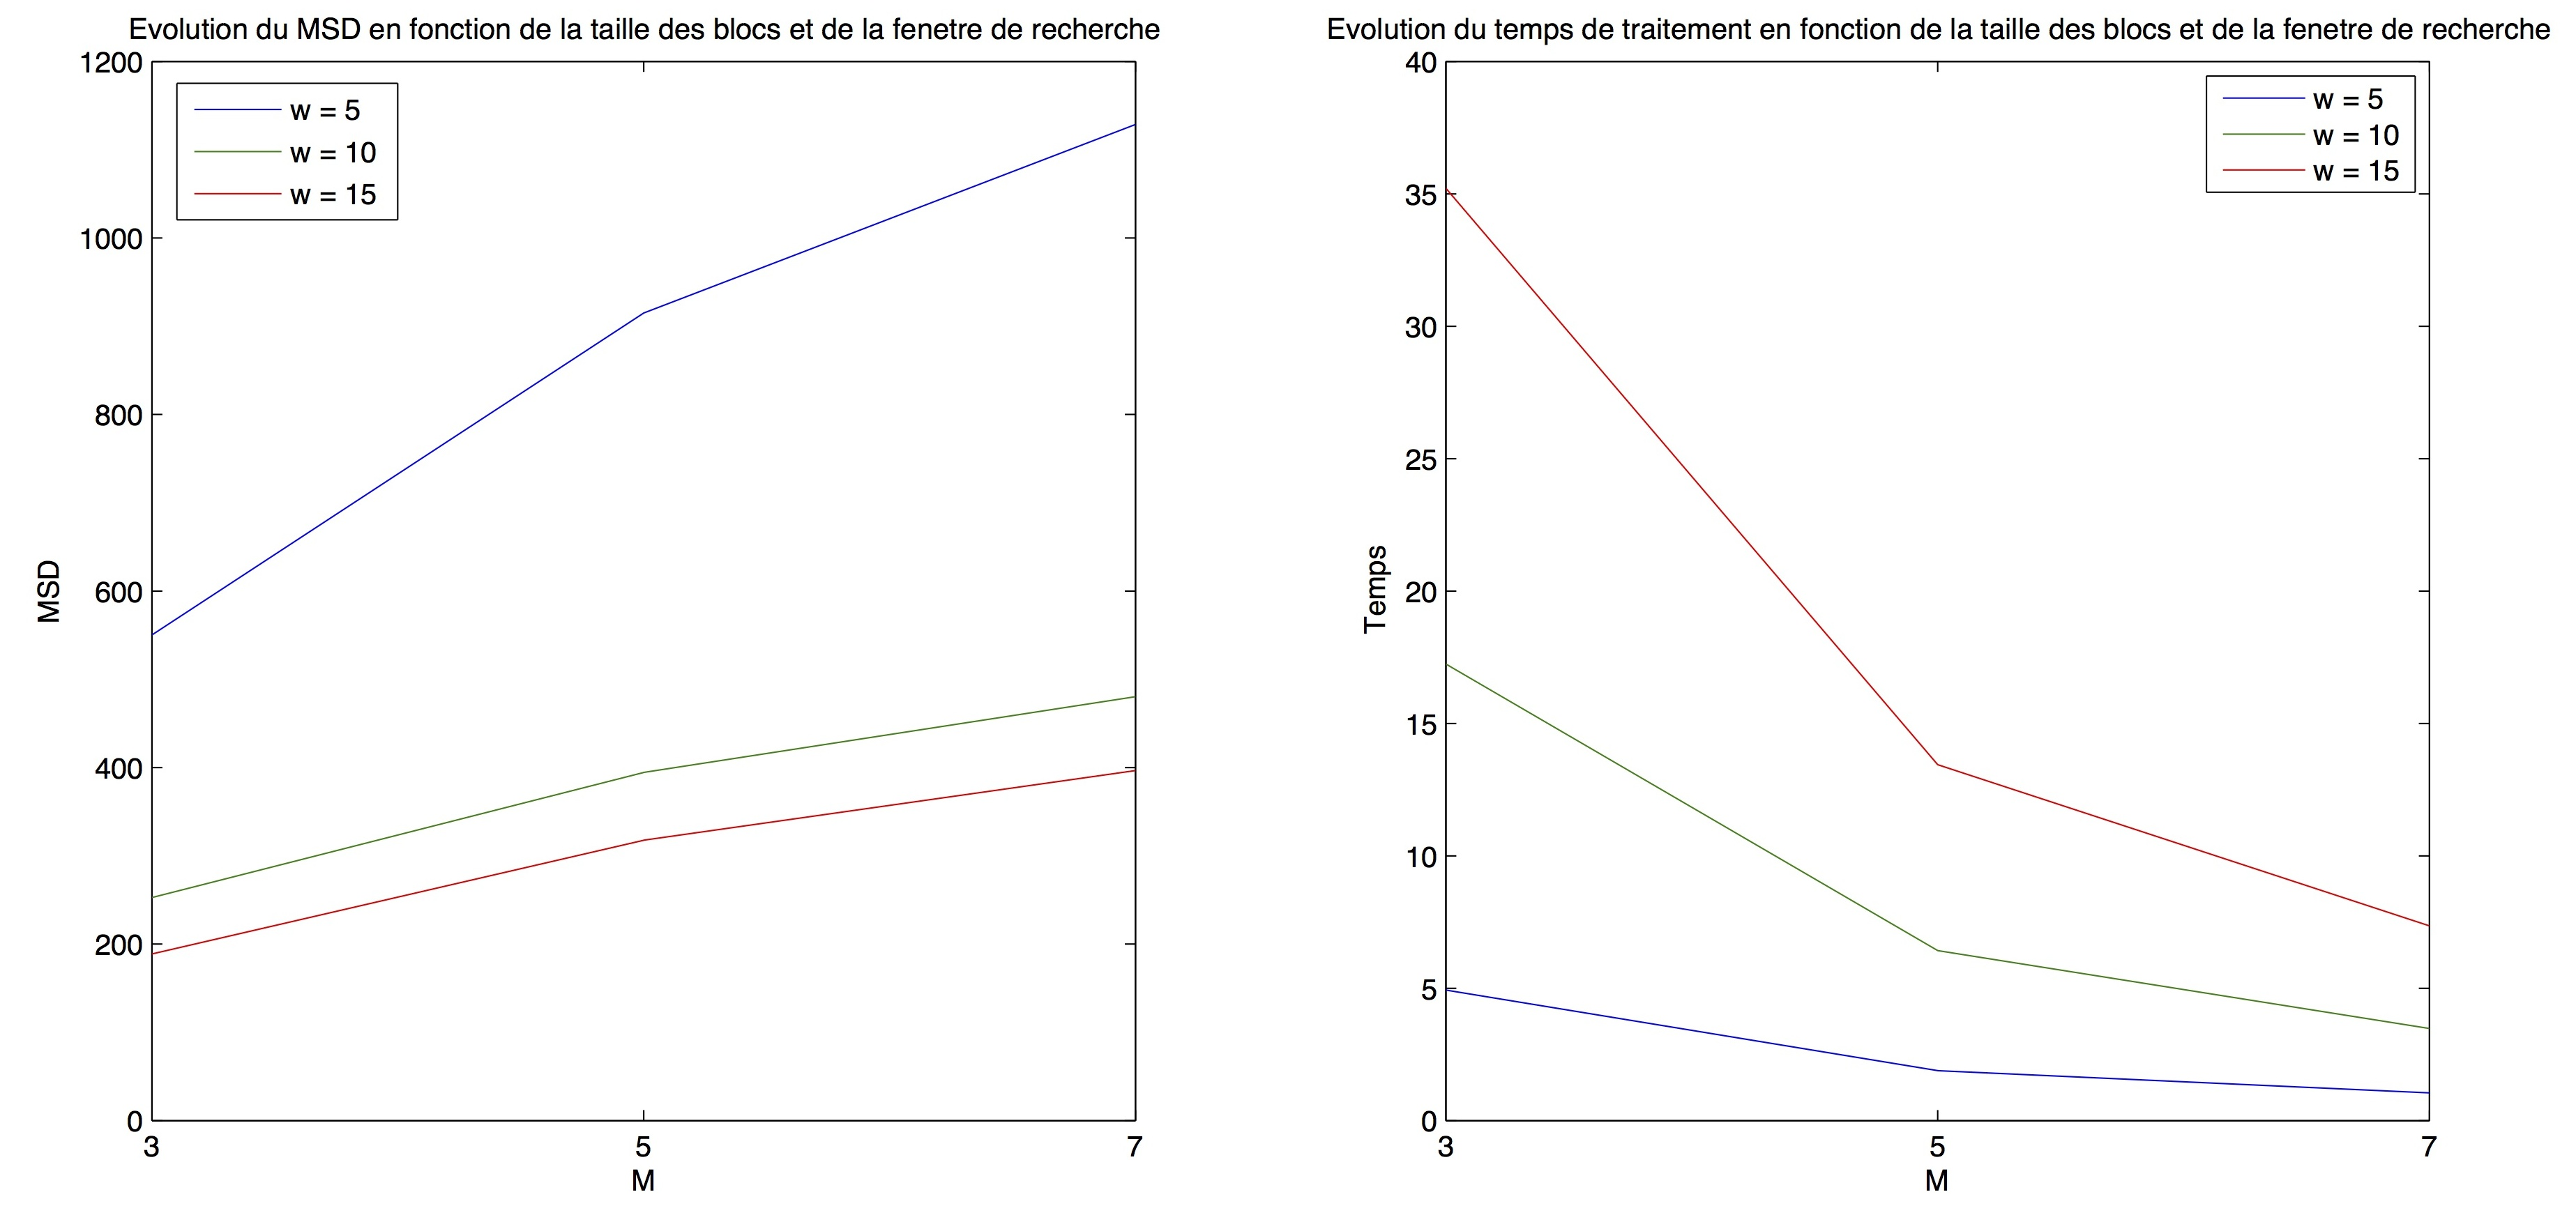
\includegraphics[height=8cm]{../Resultats/Garden/garden_graph.jpg}
	\caption{Evolution du MSD et du temps de calcul en fonction de M et W}
	\label{fig:garden_graph}
\end{figure}

On observe que plus la fenêtre de recherche est grande, plus le MSD sera faible, mais plus le temps de calcul sera important. Et inversement pour la taille des blocs. Plus les blocs seront grands, plus le MSD sera important et moins le temps de calul sera important.



\newpage

\section{Conclusion}

(Ouverture) Temps de calculs intéressants avec recherche logarithmique ou l'estimation de mouvement hiérarchique (p.49 dans le poly).

\clearpage

%
% ANNEXE
%
\appendix

\section{Codes source MATLAB}

\subsection{Calcul du MSD}\label{msd_code}

\FSource{../compute_msd.m}

\newpage

\subsection{Calcul de la fenêtre de recherche}\label{search_window}

\FSource{../search_window.m}

\newpage

\subsection{Recherche d'un bloc dans l'image de référence}\label{block_search}

\FSource{../block_matching.m}

\newpage

\subsection{Block Matching}\label{block_matching}

\FSource{../block_matching_encode.m}


\end{document}